\documentstyle[12pt,fleqn,epsfig]{aipproc}

\begin{document}
\title{Radiative Corrections -The SIMC Way}
\author{\bf{Dipangkar Dutta}}
\maketitle

\section*{Introduction}
Electrons radiate in the presence of a nuclear field due to changes in their velocity brought about by coulomb interaction and radiation resulting from
such deceleration of the electron is called Bremsstrahlung. The incoming and outgoing electrons can interact with the coulomb field of the nucleus involved in the scattering process, this results in emission and reabsorbtion of  virtual photons and emission of real soft photons. Such processes are known as internal Bremsstrahlung. The electrons can also interact with the coulomb field of a nucleus other than the one involved in the scattering process and thereby radiate photons. These radiations are known as external Bremsstrahlung. In an experiment
involving electrons scattering off some target, these radiative processes have a twofold effect on the data. Firstly the cross section of the process is modified  and secondly the kinematics (energy, momentum, angle) of the electron are also changed. Although, these are real physical processes, they are experiment specific, and so most theoretical calculations do not take 
these effects into account. Thus, in
order to get to the underlying physics, and also to directly compare with theoretical calculations, one needs to unfold these radiative processes from the data.
The procedure for doing such radiative corrections was first derived by J. Schwinger \cite{jsw}, which were later modified by Mo and Tsai \cite{mots}.  
Radiative correction formulas for coincidence $(e,e'p)$ reactions were calculated from the Mo and Tsai formulation by Makins et. al. \cite{mak1}. The derivation of these formulae is very well described in
references \cite{mak1} and \cite{mak2}, so I will not venture to write down the full derivation at this time. The goal of this paper is to elaborate on how the above mentioned formulae are used in the PWIA Monte Carlo SIMC.

\section*{Radiative Correction for Coincidence {\lowercase{\bf{\large{$(e,e'p)$}}}} Reactions}

The cross-section for radiating energy $E_{e}$ along the incoming electron direction $\hat{k}$, $E_{e^{'}}$ along the scattered electron direction $\hat{k^{'}}$, $E_{p^{'}}$ along the direction of the scattered proton $\hat{p^{'}}$ and also radiating any number of soft photons with energy less than $\Delta E $, calculated to all orders, is given by :

$$
\frac{d\sigma}{d\Omega_{e}dE_{e}dE_{e^{'}}dE_{p^{'}}} = \frac{d\sigma}
{d\Omega_{e}}\vert_{ep}(1-\delta_{hard}) \frac{\lambda_{e}\lambda_{e^{'}}
\lambda_{p^{'}}}{(\sqrt{kk^{'}})^{\lambda_{e}}(\sqrt{kk^{'}})^{\lambda_{e^{'}}}
(\sqrt{Mp^{o'}})^{\lambda_{p^{'}}}}
$$
\begin{equation}
\mbox{x}\frac{ 1 }{E_{e^{ }}^{1-\lambda_{e}}
E_{e^{'}}^{1-\lambda_{e^{'}}}E_{p^{'}}^{1-\lambda_{p^{'}}}} 
\end{equation}

Here the total energy radiated is $\omega_{total} = E_{e} + E_{e^{'}} + E_{p^{'}}$, and the $\lambda$~s are the angular distribution functions of the photons radiated in the three directions. The Angular distribution of the radiation is approximated as :

\begin{equation}
A_{peaking}(\hat{\omega}) = \lambda_{e}\delta(\hat{\omega} - \hat{k}) + \lambda_{e^{'}}\delta(\hat{\omega} - \hat{k^{'}}) + \lambda_{p^{'}}\delta(\hat{\omega} - \hat{p^{'}})
\end{equation}

This simple approach to the angular distribution is also known as the ' extended peaking approximation'. The $\lambda$~s are given by the following expressions:

\begin{equation}
\lambda_{e} = \frac{\alpha}{\pi}[ln(\frac{4k^{2}}{m^{2}} - 1)] + \frac{\alpha}{\pi}[2ln(\frac{k}{k^{'}} + ln(\frac{1 - cos\theta_{e}}{2})]
\end{equation}

\begin{equation}
\lambda_{e^{'}} = \frac{\alpha}{\pi}[ln(\frac{4k^{'2}}{m^{2}} - 1)] + \frac{\alpha}{\pi}[2ln(\frac{k}{k^{'}} + ln(\frac{1 - cos\theta_{e}}{2})]
\end{equation}

\begin{equation}
\lambda_{p^{'}} = \frac{\alpha}{\pi}[ln(\frac{p^{'o} + |p^{'}|} {p^{'o} - 
|p^{'}|}) - 2]
\end{equation}

$k, k^{'}$ and $ p^{'}$ are the magnitude of the incident electron momentum, scattered electron momentum and the scattered proton momentum respectively and $p^{'o}$ is the proton energy. $\delta_{hard}$ is the contribution from the second order virtual photon radiation to the vertex corrections, and is given by:

\begin{equation}
\delta_{hard} = 2\alpha [ - \frac{3}{4\pi} ln( -q^{2}/m^{2}) + \frac{1}{\pi} - \sum_{i}\delta_{i}^{vp}(q^{2})],
\end{equation}

where $ \sum_{i}$ sums over the different flavors of leptons with mass $m_{i}$ and,

\begin{equation}
\delta_{i}^{vp} = \frac{1}{3\pi}[ - \frac{5}{3} + ln(-q^{2}/m^{2}_{i})] 
\end{equation}

All of the above expressions are for what is known as internal Bremsstrahlung, however
photons are also emitted when the electrons are in the field of nuclei other than those involved in the hard scattering process. This is known as external
Bremsstrahlung. The proton being massive emits negligible amounts of external
radiation. Both $E_{i}^{int}$ and $E_{i}^{ext}$ are emitted in the same direction, thus if the internal and external Bremsstrahlung are added together then we can write the cross-section in terms of $E_{i}$ and $E_{f}$ radiated along $k$ and $k^{'}$ as :

$$
\frac{d\sigma}{d\Omega_{e}dE_{i}^{int}dE_{i}^{ext}dE_{f}^{int}dE_{f}^{ext}dE_{p^{'}}} = \frac{d\sigma}{d\Omega_{e}}\vert_{ep}(1-\delta_{hard})\frac{1}{\Gamma(1+bt_{i})}\frac{1}{\Gamma(1+bt_{f})}
$$
\begin{equation}
\mbox{x}\frac{(bt_{i} + \lambda_{i})}{k^{bt_{i}}
(\sqrt{kk^{'})^{\lambda_{i}}}}\frac{(bt_{f} + \lambda_{f})}{k^{'bt_{f}}(\sqrt{kk^{'})^{\lambda_{f}}}}\frac{dE_{i}}{E_{i}^{1-\lambda_{i}-bt_{i}}}\frac{dE_{f}}
{E_{f}^{1-\lambda_{f}-bt_{f}}}\Phi_{i}^{ext}(E_{i})\Phi_{f}^{ext}(E_{f})
\end{equation}

Where the function $\Phi^{ext}$ is a correction for external radiation which have large photon energies and
has the form:

\begin{equation}
          \Phi^{ext}_{i}(E_{i}) = 1 - \frac{bt_{i}}{bt_{i}+ \lambda_{i}}\frac{E_{i}}{k_{i}}
\end{equation}

and

\begin{equation}
         b = 1/9(12 + \frac{ Z + 1}{ ZL_{1} + L_{2}})
\end{equation}

\begin{equation} 
        L_{1} = ln(184.15) - \frac{1}{3}ln(Z)
\end{equation}

\begin{equation}
        L_{2} = ln(1194.)  - \frac{2}{3}ln(Z)
\end{equation}



\section*{The Radiative Correction Procedure in The PWIA Monte Carlo SIMC}

In the Monte Carlo SIMC the photon energies $E_{e}, E_{e'}$ and $E_{p'}$ along the incoming electron, the outgoing electron and the proton directions respectively, are generated separately. The total energy energy radiated is the
vector sum as given by equation $2$. This comes about because in 
equation $1$ above we notice that the energy and angular distribution of 
 radiation in the three directions factorize into three independent functions. 

The shape of each of these distributions has the form:

\begin{equation}
\frac{1}{\Gamma(1+bt)}\frac{bt+\lambda}{k^{bt}(\sqrt{kk^{'}})^{\lambda}}\frac{dE}{E^{1-\lambda-bt}}
\end{equation}

If we rename $bt+ \lambda$ as g and $\frac{bt+\lambda}{\Gamma(1+bt)}\frac{1}{k^{bt}(\sqrt{kk'})^{\lambda}} $ as C we get the simple form:

\begin{equation}
 C*E^{g-1}dE
\end{equation}

Hence we can use this simple form to generate the energy radiated in a given direction
between limits $E_{max}$ and $E_{min}$. The generating function must normalize to 1 between these limits so we have 
\begin{equation}
N*\int^{E_{max}}_{E_{min}}(E^{g-1})dE = 1
\end{equation}

or

\begin{equation}
N= \frac{g}{E_{max}^{g} - E_{min}^{g}}
\end{equation}

Thus for each of the radiation tails, the energy radiated in that particular
direction is randomly generated in the range $E_{max} - E_{min}$ using the 
generating function or energy shape:

\begin{equation}
G = \frac{gE^{g-1}}{E_{max}^{g} - E_{min}^{g}}
\end{equation}


The limits $E_{max}$ and $E_{min}$ are determined from the limits of the model spectral function, the limits on the energy and momenta of the incident and scattered particles determined from the spectrometer acceptance and the randomly generated energy and momenta of the incident and scattered particles.

Once the energy radiated in each of the tails is known, the next step is to use these energies to modify the momentum and energy of the incident and scattered particles involved in the reaction. This is done for each event by subtracting off the radiated energy from the randomly generated vertex energies (energy of the particles at the reaction vertex). 

Next the radiation weight is calculated for each event which is then assigned
to that event. The radiation weight is the probability of radiating soft or hard photons of a given energy. The radiation weight had three components. The first component is the probability of emitting a photon which has the correct
radiative tail shape, this comes from equation $13$ and the generating function (equation $17$). From these equations we get the weight for each of the three tails as:  

\begin{equation}
W_{rad}^{i} = C/g *((E^{i}_{max})^{g} - (E^{i}_{min})^{g}); i=e,e',p' 
\end{equation}

 
The product of the three weights for the three tails give us 
$W_{rad}^{soft}$. 

\begin{equation}
W_{rad}^{soft} = W_{rad}^{e}W_{rad}^{e{'}}W_{rad}^{p^{'}}
\end{equation}

The second  component is the multiplicative correction 
factor due to external  radiation $\Phi^{ext}_{i}$, as described in equation $9$. This too is calculated for each tail. The final component is the
due to the vertex corrections and is given by $(1-\delta_{hard})$. So finally
the product of all these little pieces gives us the radiation weight for an event.

\begin{equation}
W_{rad}^{event} = W_{rad}^{soft}\Phi^{ext}_{e}\Phi^{ext}_{e'}\Phi^{ext}_{p'}(1-\delta_{hard})
\end{equation}


When the data is binned in terms of $E_{m}$ and $P_{m}$, we have  
accounted for events which radiated into a particular bin by modifying the vertex. The $E_{m}$ and $P_{m}$ was changed by exactly the total radiated energy, hence they contribute to bins they radiated into and not the ones they would have if there was no radiation. In addition the
radiation weight assigned to each event accounts for events which radiated out of the bin. These two features together constitute the radiative correction procedure of the Monte Carlo SIMC. Thus using the described procedure we can generate radiated spectra with SIMC. This method
obtains correct multi-photon angular distributions and hence is also known as 
the 'multi-photon' technique. However, one must remember that it does involve 
the peaking approximation at the single photon level. 

As an illustration of how the procedure works, Fig 1 compares an unradiated
missing energy vs missing momentum spectrum with a radiated spectrum for 
Hydrogen target. One can clearly identify  the radiative tails in this figure. 
In Fig 2 the hydrogen missing energy spectrum is compared with the same 
calculated using the Monte Carlo.

\begin{figure}  
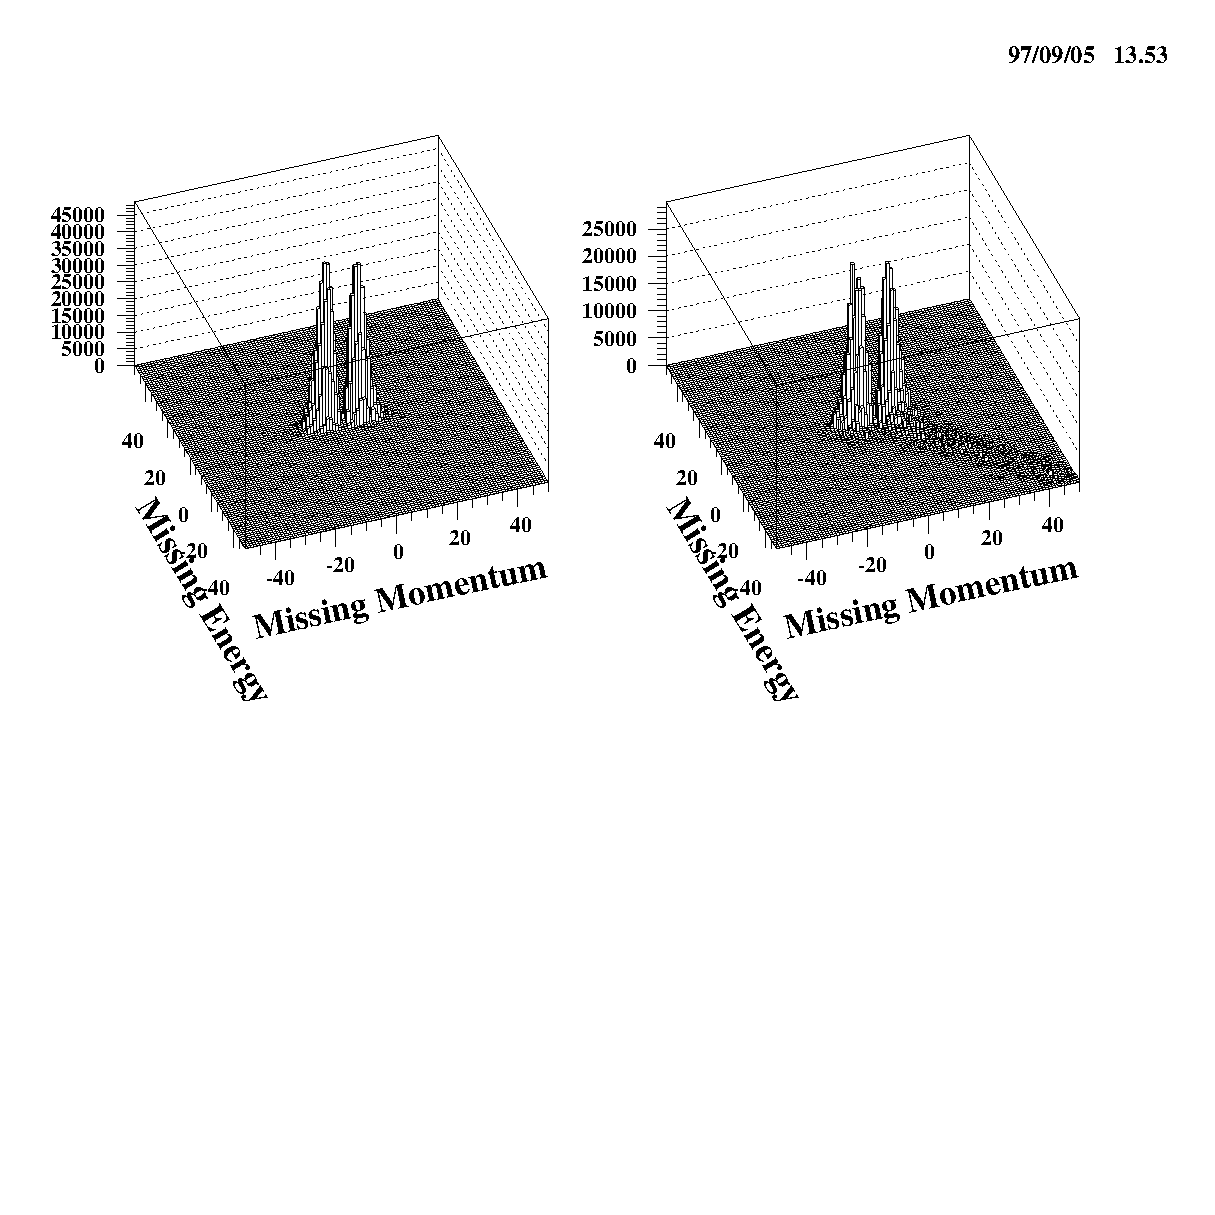
\epsfig{file=rad.eps,height=7in,width=7in}
\vspace{10pt}
\caption{Plot of missing energy vs missing momentum for hydrogen with and without radiation.}
\end{figure}




\begin{figure}  
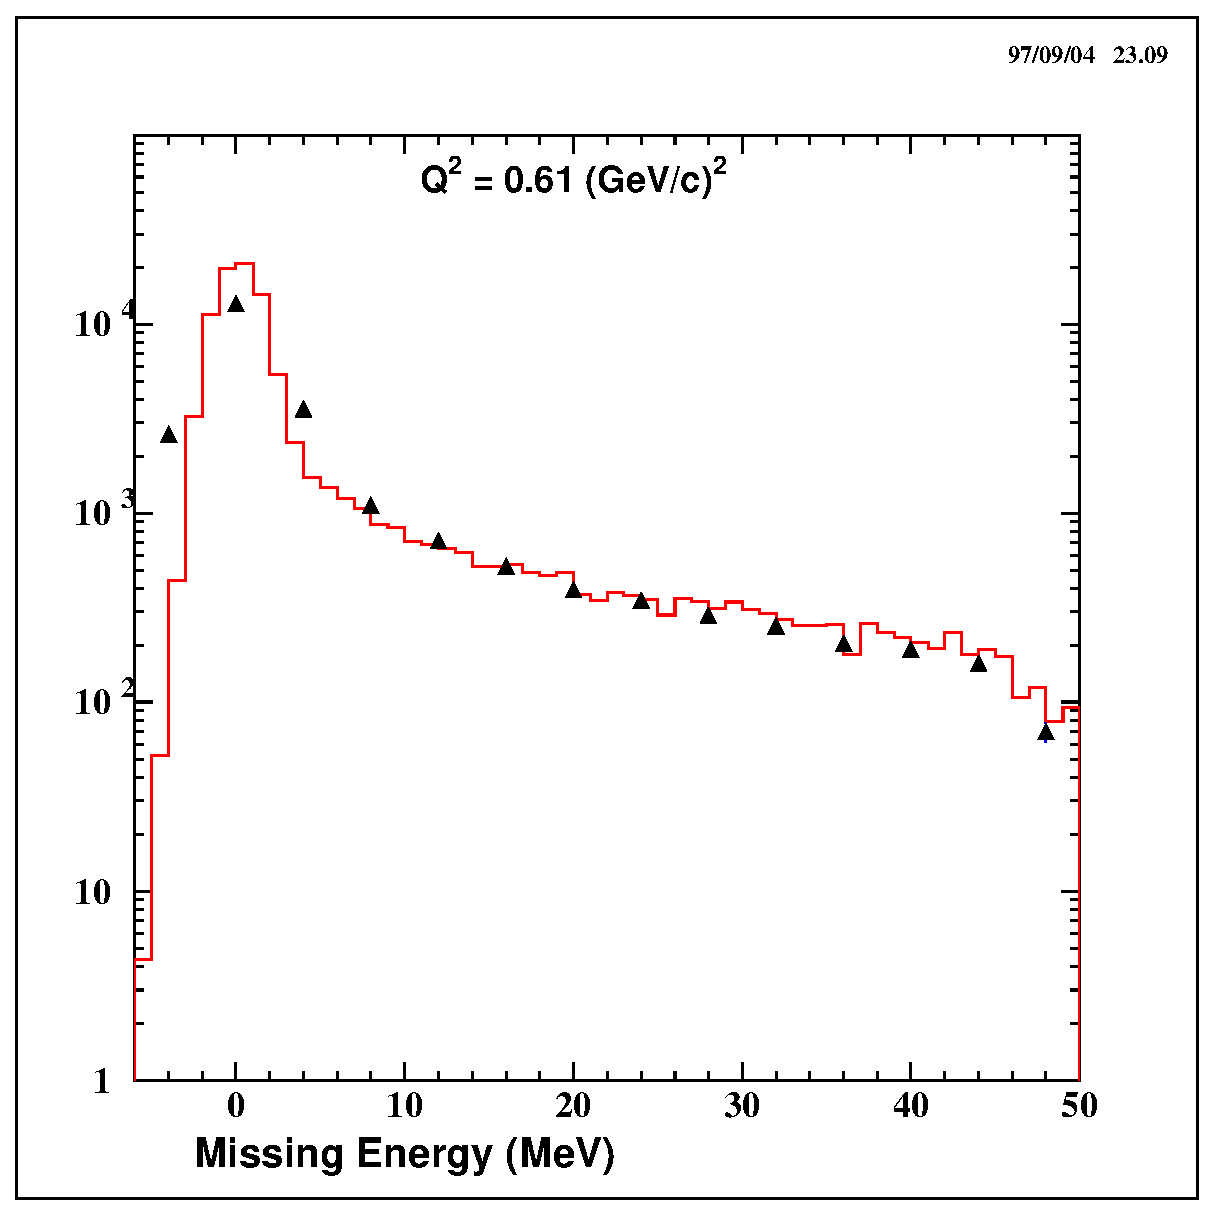
\epsfig{file=radcomprd.eps,height=7in,width=7in}
\vspace{10pt}
\caption{Plot of the missing energy spectrum of hydrogen, solid line is the calculation using Monte Carlo SIMC and triangles are data, with statistical errors only.}
\end{figure}


\section*{Conclusions}
The procedure described above is one of the three radiative correction 
procedures which are available in SIMC. The procedure described is the 
one currently in use. Various comparisons of the different procedures were
done by the authors and they found agreement to be better than $1\%$ within the different procedures. Since the above procedure approximates the angular distribution most effectively, it is the procedure of choice. 


\begin{references}
\bibitem{jsw}J. Schwinger, {\it Phys.\ Rev.\ } {\bf 76}, 790 (1949). 
\bibitem{mak1}N.C.R.Makins, Massachusetts Institute of Technology Ph.D. thesis (1994).
\bibitem{mots}L.W. Mo, Y.S. Tsai, {\it Revs. Mod. Phy.} {\bf 41}, 205 (1969).
\bibitem{mak2}N.C.R. Makins et al., Radiative Corrections for $(e,e'p)$ Reactions, (1994) Unpublished.
\end{references}   


\end{document}




